%%%%%%%%%%%%%%%%%%%%%%%%%%%%%%%%%%%%%%%%%
% a0poster Landscape Poster
% LaTeX Template
% Version 1.0 (22/06/13)
%
% The a0poster class was created by:
% Gerlinde Kettl and Matthias Weiser (tex@kettl.de)
%
% This template has been downloaded from:
% http://www.LaTeXTemplates.com
%
% License:
% CC BY-NC-SA 3.0 (http://creativecommons.org/licenses/by-nc-sa/3.0/)
%
%%%%%%%%%%%%%%%%%%%%%%%%%%%%%%%%%%%%%%%%%

%----------------------------------------------------------------------------------------
%	PACKAGES AND OTHER DOCUMENT CONFIGURATIONS
%----------------------------------------------------------------------------------------

\documentclass[a0,landscape]{a0poster}

\usepackage{multicol} % This is so we can have multiple columns of text side-by-side
\columnsep=80pt % This is the amount of white space between the columns in the poster
\columnseprule=1pt % This is the thickness of the black line between the columns in the poster

\usepackage[svgnames]{xcolor} % Specify colors by their 'svgnames', for a full list of all colors available see here: http://www.latextemplates.com/svgnames-colors

\usepackage{times} % Use the times font
%\usepackage{palatino} % Uncomment to use the Palatino font

\usepackage{graphicx} % Required for including images
\graphicspath{{figures/}} % Location of the graphics files
\usepackage{booktabs} % Top and bottom rules for table
\usepackage{siunitx}

\usepackage[font=small,labelfont=bf]{caption} % Required for specifying captions to tables and figures
\usepackage{amsfonts, amsmath, amsthm, amssymb} % For math fonts, symbols and environments

\usepackage{wrapfig} % Allows wrapping text around tables and figures

\usepackage{supertabular}

\usepackage{hyperref}

\usepackage[utf8]{inputenc} % Pour utiliser les caractères accentués
\usepackage{tikz}
\usetikzlibrary{shapes}
\usetikzlibrary{positioning}
\usepackage[export]{adjustbox}
\usepackage[skins,listings,breakable,listingsutf8,theorems,hooks,fitting]{tcolorbox}
\usepackage[round]{natbib}
\tcbuselibrary{raster}


\usepackage{float}


% constants
\newcommand{\vspacebetweenbullets}{0.25cm}
\newcommand{\vspacebetweensubsections}{2cm}
\newcommand{\hspacefigandtext}{0.5cm}





\begin{document}

%----------------------------------------------------------------------------------------
%	POSTER HEADER
%----------------------------------------------------------------------------------------

% The header is divided into three boxes:
% The first is 55% wide and houses the title, subtitle, names and university/organization
% The second is 25% wide and houses contact information
% The third is 19% wide and houses a logo for your university/organization or a photo of you
% The widths of these boxes can be easily edited to accommodate your content as you see fit

\noindent\begin{minipage}[b]{\linewidth}
\centering
\noindent \veryHuge \color{NavyBlue} \textbf{Projected changes to hydrometeorologic extremes across Canada} \color{Black}\\ % Title
\noindent\begin{minipage}[c]{0.2\linewidth}
      \center
      
\includegraphics[width=25cm]{logo_cnrcwp_escer.png} % Logo or a photo of you, adjust its dimensions here
\end{minipage} \hfill
%
\begin{minipage}[c]{0.15\linewidth}
  \center
  \Large \textbf{Oleksandr Huziy} \\
  \large \texttt{guziy.sasha@gmail.com}
\end{minipage}
%
\begin{minipage}[b]{0.01\linewidth}
 \center
 \Large\&
\end{minipage}
%
\begin{minipage}[c]{0.15\linewidth}
   \center
   \Large \textbf{Dae Il Jeong} \\
   \large  \texttt{dae.jeong2@gmail.com}
\end{minipage}\hfill
%
\begin{minipage}[b]{0.01\linewidth}
 \center
 \Large\&
\end{minipage}
%
\begin{minipage}[c]{0.15\linewidth}
   \center
   \Large \textbf{Laxmi Sushama} \\
   \large  \texttt{sushama.laxmi@uqam.ca}
\end{minipage}\hfill
%
\begin{minipage}[c]{0.2\linewidth}
  \center
  
\includegraphics[width=10cm]{logo_uqam.png} % Logo or a photo of you, adjust its dimensions here
\end{minipage}
\rule{\linewidth}{3pt}
\end{minipage}
%

\vspace{0.1cm} % A bit of extra whitespace between the header and poster content

%----------------------------------------------------------------------------------------

\begin{multicols*}{4} % This is how many columns your poster will be broken into, a poster with many figures may benefit from less columns whereas a text-heavy poster benefits from more

%----------------------------------------------------------------------------------------
%	INTRODUCTION
%----------------------------------------------------------------------------------------

\color{DarkSlateGray} % SaddleBrown color for the introduction

\section*{(A) Introduction}
The Fifth Assessment Report of the Intergovernmental Panel on Climate Change
concluded that there will be an intensification of the hydrological cycle in the
future warmer climate. It was also reported that the frequency and intensity of
extreme precipitation events have likely increased over North America and Europe
since around 1950 \citep{hartmann2013} and that it will very likely increase
over most mid-latitude land-masses in future climate \citep{collins2013}.

In this study the changes in hydro-meteorological extremes are assessed over
Canada, using transient climate change simulations of the fifth generation of
Canadian Regional Climate (CRCM5) model. Specifically, the results are reported
on changes to the rain on snow events over North America \citep{jeong2016ros}, heat wave events over
Canada \citep{jeong2016heatwave}, high and low flow streamflow values \citep{jeong2014copula,huziy2016impact} both using
univariate and multivariate analysis over northeastern Canadian watersheds.



%----------------------------------------------------------------------------------------
%	OBJECTIVES
%----------------------------------------------------------------------------------------

\color{DarkSlateGray} % DarkSlateGray color for the rest of the content

\section*{(B) Main Objectives}
\begin{tcolorbox}[colback=white,colframe=green!40!black]
  \color{DarkSlateGray}
  \begin{enumerate}
    \item Summarize our recent results on projected changes to characteristics of hydrometeorologic extremes.
    \item Analyze links and coherency of climate change projections from different experiment configurations.
  \end{enumerate}
\end{tcolorbox}

%----------------------------------------------------------------------------------------
%	MATERIALS AND METHODS
%----------------------------------------------------------------------------------------

\section*{(C) Methods and experiment configurations}
\subsection*{C.1 Methods}
%
\begin{itemize}
  \item (D.1) ROS day:  a day with both liquid precipitation and SWE above 1mm
  \item (D.2) Heat wave event: a period of three or more consecutive days of Tmax at or above the absolute temperature threshold of 32$^\circ$C
  \item (D.3) The Generalized Extreme Value (GEV) distribution is used to compute return
        levels of extreme ({\color{red} high} and {\color{blue}low}) flow events. The {\color{red} high} ({\color{blue}low}) flow event is
        defined as the maximum (minimum) 1-day (15-day) flow occurring during the \textbf{March}
        to \textbf{July} (\textbf{January} to \textbf{May}) period. Statistical significance of the projected
        changes to the {\color{red} high} and {\color{blue}low} flow return levels at the 5\%
        significance level is determined using the non-parametric vector bootstrap
        resampling method.
  \item (D.4) Multivariate analysis using Copula: Links univariate marginal distribution
         functions (Generalized Extreme Value distribution, GEV) to form a multivariate
        distribution function (Clayton family).
\end{itemize}

\subsection*{C.2 Experiment setup}
\begin{center}
  \small
  \begin{supertabular}{ccccl} \toprule
      Section & $\Delta x$ & Current period & Future Period & Additional information \\ \toprule
      D.1    & 0.4$^\circ$ & 1976-2005      & 2041-2070     & \begin{minipage}[t]{8cm}\flushleft CRCM5 and CanRCM4, RCP85 scenario\vspace{0.8cm} \end{minipage}\\
      D.2    & 0.4$^\circ$ & 1970-1999      & 2040-2069     & \begin{minipage}[t]{8cm}\flushleft NARCCAP (North American Regional Climate Change Assessment Program), A2 scenario\vspace{0.8cm} \end{minipage}\\
      D.3    & 0.1$^\circ$ & 1980-2010      & 2070-2100     & \begin{minipage}[t]{8cm}\flushleft lakes: Hostetler, rivers: WATROUTE-modified\vspace{0.8cm} \end{minipage}\\
      D.4    & 0.4$^\circ$ & 1970-1999      & 2041-2070     & \begin{minipage}[t]{8cm}\flushleft Ensemble of CRCM4 simulations, WATROUTE-offline, A2 scenario\vspace{0.8cm} \end{minipage}\\
      \bottomrule
  \end{supertabular}

  \vspace{1cm}
  \begin{minipage}{\linewidth}
   *If not specified, atmosphere is modelled using various CRCM (Canadian Regional Climate Model) model. CanRCM4 (ECCC/CCCma) is used only in (D.1).
  \end{minipage}
\end{center}


%----------------------------------------------------------------------------------------
%	RESULTS
%----------------------------------------------------------------------------------------

\section*{(D) Results}

\subsection*{D.1 Rain on snow events over North America \citep{jeong2016ros}}
\begin{center}
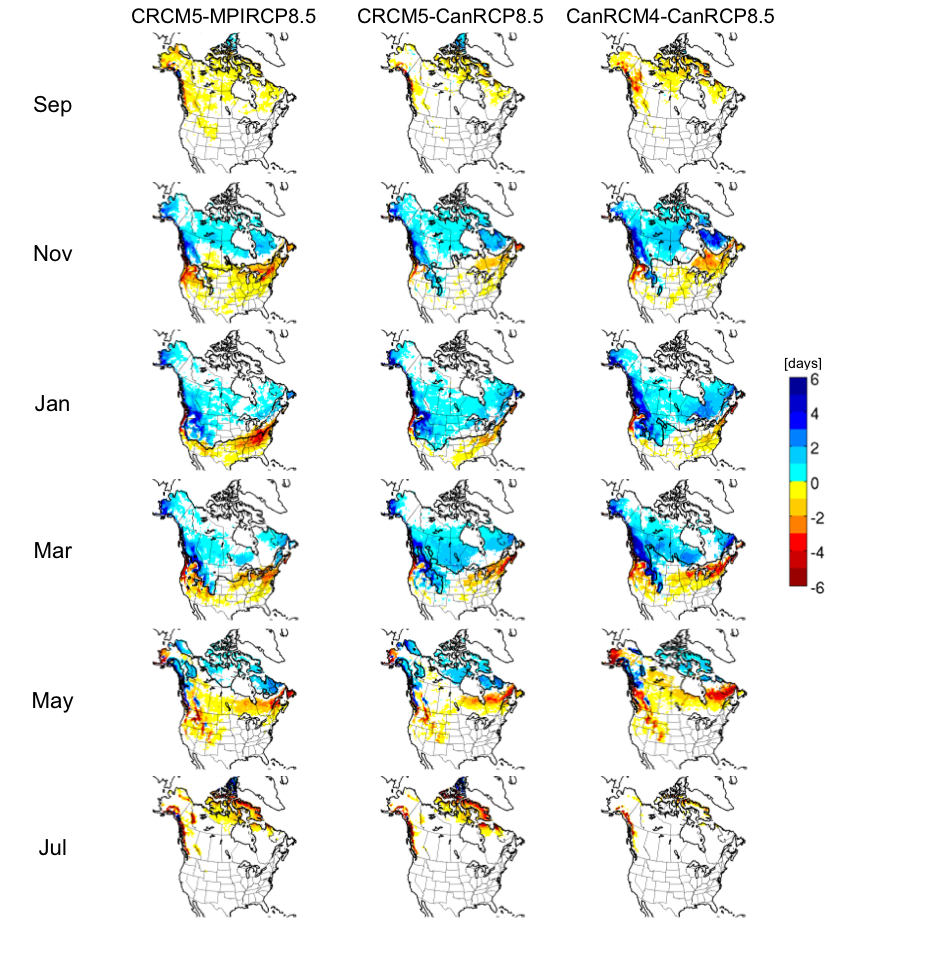
\includegraphics[width=0.6\linewidth]{cc_num_of_ros}
\captionof{figure}{\label{fig_cc_num_of_ros}\color{Green} Projected changes to the number of ROS days for the three RCM simulations (i.e.,
                                CRCM5-MPIRCP8.5, CRCM5-CanRCP8.5, and CanRCM4-CanRCP8.5) for the future
                                2041-2070 period with respect to the current1976-2005 period. The black contour
                                represents the mean freezing line in future climate. Projected changes are shown
                                when they are statistically significant with the two-sample t-test at the 10\%
                                significance level.}
\end{center}
$\bullet$ The three simulations suggest general increases in the future ROS
characteristics to the north of the future freezing line due to increases in
rainfall frequency with increased air temperature \\[\vspacebetweenbullets]
$\bullet$ They suggest general decreases in future ROS characteristics to the south of the
future freezing line due to decreases in SWE and snow cover frequency in future
climate \\[\vspacebetweenbullets]
$\bullet$ Consequently, they generally suggest increases in future ROS characteristics
during the November to March period for most regions of Canada and northwestern US

\subsection*{D.2 Heat wave events over Canada \citep{jeong2016heatwave}}
\begin{center}
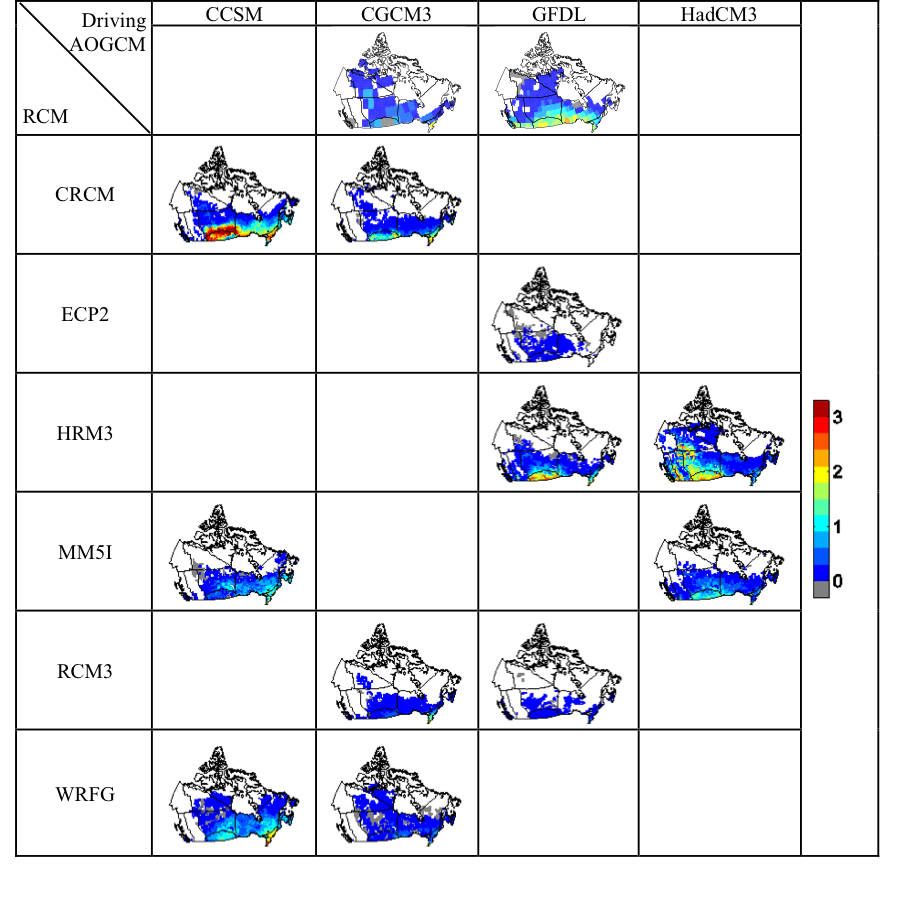
\includegraphics[width=0.6\linewidth]{cc_heatwaves}
\captionof{figure}{\label{fig_cc_heatwaves}\color{Green} Projected changes to the number of heat wave events per summer (JJA) for the 2 driving
                                AOGCMs and 11 RCM-AOGCMs for the future 2040–2069 period with respect to the
                                current 1970–1999 period. Grid points are colorless if simulations do not yield
                                any heat wave event for both periods.}
\end{center}
$\bullet$ Projected changes are robust as all RCM-AOGCMs suggest an increase for southern Canada, where the 90th percentile of Tmax almost reached 32$^\circ$C in summer \\[\vspacebetweenbullets]
$\bullet$ On average, RCM-AOGCMs suggest the largest increase in NPLAINS and the second largest increase in GRTLKS \\[\vspacebetweenbullets]
$\bullet$ Several RCM-AOGCMs (i.e., HRM3-GFDL, HRM3-HadCM3, RCM3-CGCM3, and RCM3-GFDL)
      tend to underestimate projected changes in the heat wave events, especially in
      the southeastern Canadian climatic regions, due to cold biases in Tmax

\subsection*{D.3 Projected changes to high and low flow return levels for major Quebec watersheds \citep{huziy2016impact}}
\begin{center}
  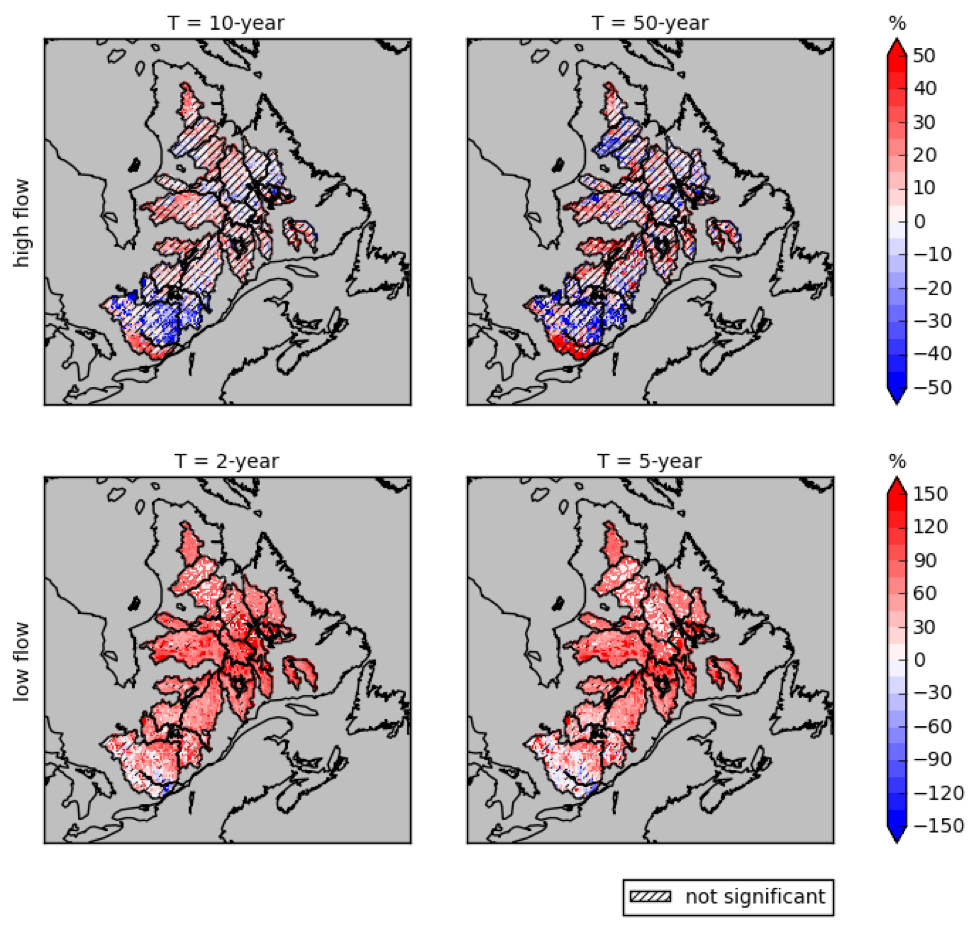
\includegraphics[width=0.6\linewidth]{extreme_low_and_high_flow_RL}
  \captionof{figure}{\color{Green}
  Projected changes for the 2070–2100 period with respect to the 1980-2010 period
  to the 10- and 50-year return levels of 1-day high flow (upper panel) and of 2-
  and 5-year return levels of 15-day low flow (bottom panel) for CanESM2-CRCM5-L.
  Changes that are not significant at the 5\% significance level (evaluated using
  bootstrap procedure) are hatched over.}
\end{center}
$\bullet$ Almost no significant changes to high flow return levels are detected for future climate. \\[\vspacebetweenbullets]
$\bullet$ The changes to the low flow return levels are mostly positive and significant at the 5\% significance level over all studied watersheds. \\[\vspacebetweenbullets]
$\bullet$ Some decreases to the low flow return levels are noted in the southern part of
      the domain, which might indicate reduced groundwater contribution to streamflows
      during low flow periods at those points in future climate due to enhanced summer
      evaporation and reduced summer and fall precipitation.

\subsection*{D.4 Extreme flow characteristics for Quebec watersheds based on a multivariate distribution \citep{jeong2014copula}}
\begin{center}
   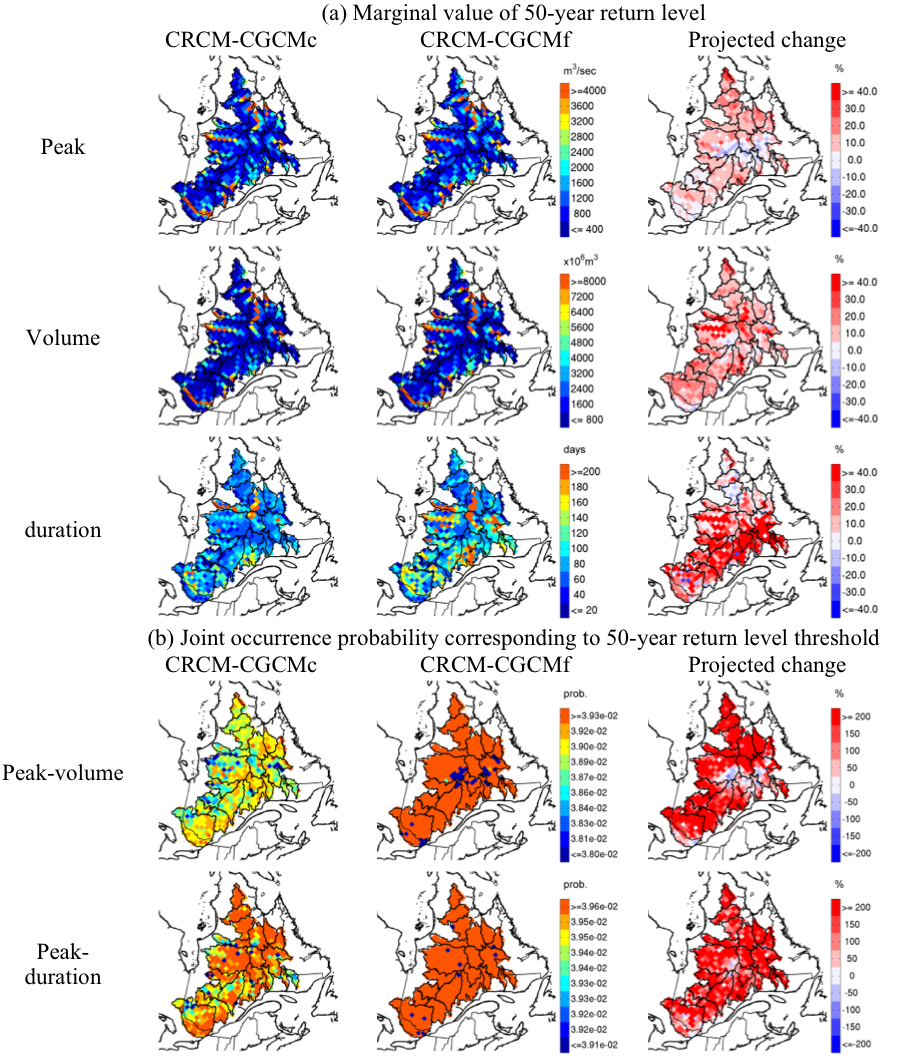
\includegraphics[width=0.6\linewidth]{cc_copula}
\end{center}

\captionof{figure}{\label{fig_cc_copula}\color{Green} Fifty-year return levels of (a) peak, volume and duration and their joint
            occurrence probabilities computed using merged longer samples for CRCM-CGCMc
            (column 1) and CRCM-CGCMf (column 2). Percentage difference between CRCM-CGCMf
            and CRCM-CGCMc is shown in column 3.}
$\bullet$ The projected changes to marginal 50-year return levels of flood peak, volume and duration suggest increases in future climate. \\[\vspacebetweenbullets]
$\bullet$ The projected increases in the flood peak, volume and duration for the majority
of the basins are caused by increased winter and spring precipitation and warmer
spring temperatures, leading to increased spring snowmelt in future climate. \\[\vspacebetweenbullets]
$\bullet$ Projected changes to joint occurrence probabilities of 50-year return levels for
the peak-volume, peak-duration and volume-duration pairs of flood
characteristics are suggested to increases in future climate.

%----------------------------------------------------------------------------------------
%	CONCLUSIONS
%----------------------------------------------------------------------------------------

\color{SaddleBrown} % SaddleBrown color for the conclusions to make them stand out

\section*{(E) Conclusions}
\begin{minipage}[t]{\linewidth}
\begin{itemize}
\item D.1 and D.3: Increased low flow values in D.3 agree with
the shortening of the cold period and increased fraction of liquid precipitation
projected in D.1.

\item D.2 and D.3: Increased number of heat wave in D.2 is
in-line with the decreasing low flow amplitudes in the southern part of the
domain.

\item D.3 and D.4: Differences in projected changes to the 50-year return levels
of high flows highlight the importance of assessing uncertainties associated
with physical parameterizations, driving data and resolution used for transient
climate change runs.

\item Simulations over bigger regions and the complete analysis of both
atmospheric fields and streamflows are required to further improve our
confidence in the relationships between projected changes to the parameters of
hydrometeorologic extremes.
\end{itemize}
\end{minipage}
\color{DarkSlateGray} % Set the color back to DarkSlateGray for the rest of the content


 %----------------------------------------------------------------------------------------
%	REFERENCES
%----------------------------------------------------------------------------------------

%\nocite{*} % Print all references regardless of whether they were cited in the poster or not
\bibliographystyle{agu} % Plain referencing style
\bibliography{sample} % Use the example bibliography file sample.bib

%----------------------------------------------------------------------------------------
%	ACKNOWLEDGEMENTS
%----------------------------------------------------------------------------------------
\section*{Acknowledgements}
This research was carried out within the Canadian Network for Regional Climate and Weather Processes (CNRCWP) project funded by the Natural Sciences and Engineering Research Council (NSERC) of Canada.
%----------------------------------------------------------------------------------------

\vfill
\begin{tcolorbox}[colback=red!5!white,colframe=red!75!black,title=Additional information]
Interested in CNRCWP activities?

Visit our website and subscribe to our twitter account:
\tcblower
\begin{itemize}
  \item webpage: \href{http://cnrcwp.uqam.ca}{http://cnrcwp.uqam.ca}
  \item twitter: \href{http://twitter.com/cnrcwp}{http://twitter.com/cnrcwp}
\end{itemize}
\end{tcolorbox}
%



\end{multicols*}
\end{document}
